% @AML: Once flow of paper, overall message, etc is decided, we'll most likely want to change this sub-heading
% @AML: Todo - update metric names to be consistent with rest of the paper.
\subsection{Tag-matching in a genetic programming context}

\begin{figure*}
  \begin{center}

  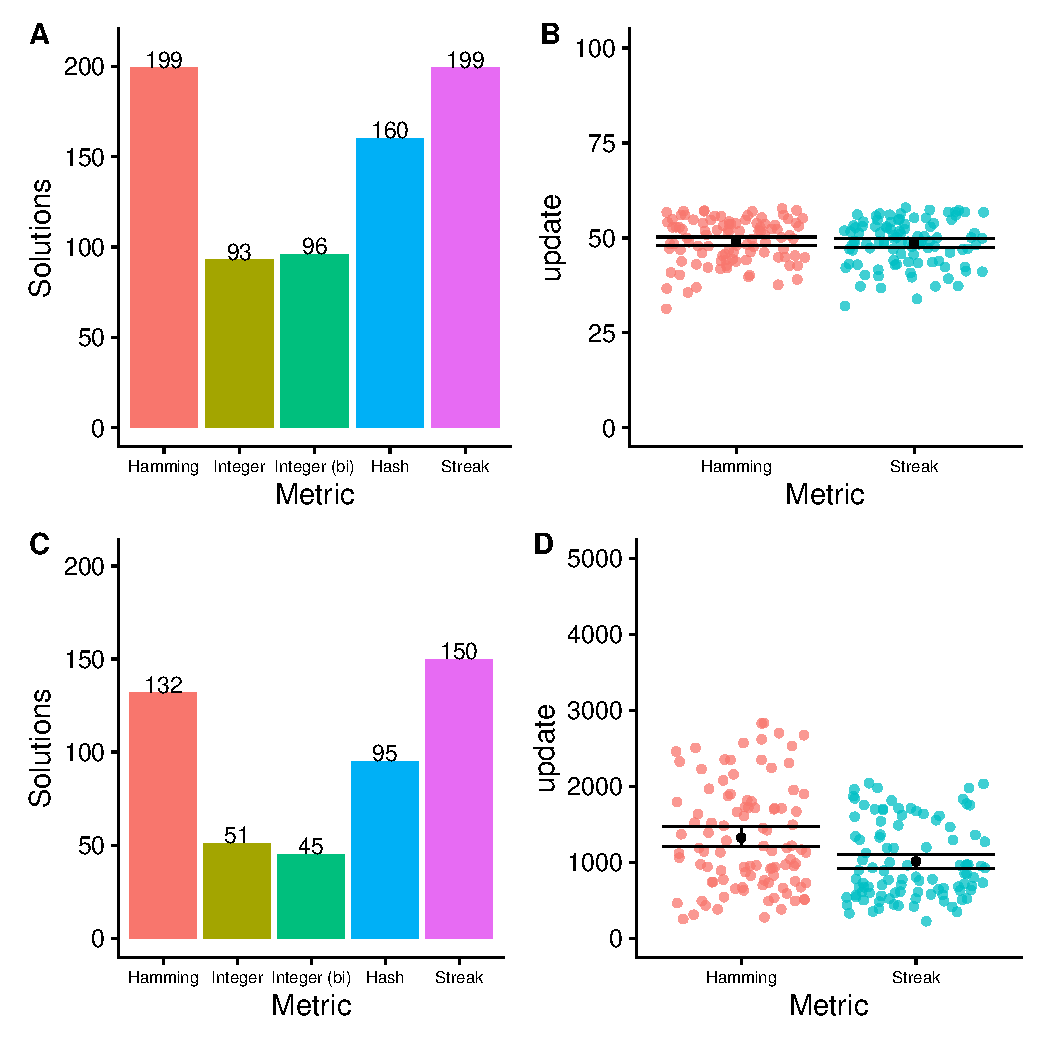
\includegraphics[width=\columnwidth]{img/gp_results/gp_results_panel}
  \caption{
  Todo - caption. A, B are changing-signal task; C, D are directional signal task.
  }
  \label{fig:gp_results}

  \end{center}
  \end{figure*}

Figure [X] gives the number of replicates that produced a successful SignalGP program (i.e., capable of achieving maximum fitness) for each tag-matching metric on both the changing- and directional-signal tasks.
For each task, we used a pairwise Fisher's exact test (with a Holm correction for multiple comparisons) to compare the number of successful replicates of each metric.
Our data and fully detailed statistical results are given in our supplemental material [cite - SGP supplement].

We observed no difference in success between the integer and integer-symmetric metrics on both the changing- and directional-signal tasks.
[Statement about consistency with expectations based on previous tag-matching experiments].
% - Appears to be consistent with results from graph matching evolution experiment. Needs confirmation, though.
% - Interesting that these two metrics seem to have fairly different geometric properties (because wrap-around vs no wrap-around), but have fairly similar variational properties.
% - For GP problems here, wrap-around vs no wrap around seems to not make a difference.

Across both tasks, the streak and hamming metrics performed significantly better than all other metrics ([STATS]).
On the changing-signal task, the hamming and streak metrics performed identically.
However, on the directional-signal task, the streak metric performed significantly better than the hamming metric ([STATS]).
To assess whether the streak metric produced solutions in fewer generations than the hamming metric, we re-ran 200 replicates of each condition (with new random number seeds) until a solution evolved in each of 50\% of the replicates (Figure [X]).
We found no difference between the hamming and streak metrics in the number generations elapsed before a solution to the changing-signal task evolves.
On the directional-signal task, however, we found that streak metric generally resulted required fewer generations for a solution to evolve than the hamming metric (Wilcoxon rank-sum test, $p < 0.0016$)
% TODO - double check that result in analyses
[Statement about consistency with expectations based on previous tag-matching experiments].
% Seems largely consistent with mean-degree-2 results (for later updates) in graph matching evolution experiment.
% More work to be done, but these data indicate that streak metric can be used for best/consistent performance in GP.

Surprisingly, the Hash metric performed well on both diagnostic tasks, outperforming both the integer and integer-symmetric metrics ([STATS?]).
The hash metric roughly maximizes the amount of phenotypic variation (i.e., signal-function relationships) that can be generated by mutating a single genotype --- a single bit flip in a tag is likely to completely re-order which other tags it best matches with.
The capacity to quickly generate large amounts of phenotypic variation allows evolution to explore a large swaths of the fitness landscape from generation to generation.
However, this capacity to generate phenotypic variation trades off with tag-matching robustness --- a single mutation to a tag is likely to destroy any established relationships with other tags.
Of each of the metrics we explored, the hash metric is the most susceptible to mutational meltdowns at high mutation rates.

% [Statement about consistency with expectations based on previous tag-matching experiments].
% [Statement about how Hash metric is good at exploring lots of combinations very quickly, with a low enough mutation rate].


% [Statement about these results overall in context of other results?].
% More work to be done, but these data indicate that streak metric can be used for best/consistent performance in GP.

